% Created 2014-06-23 Mon 00:00
\documentclass[bigger]{beamer}
\usepackage[utf8]{inputenc}
\usepackage[T1]{fontenc}
\usepackage{fixltx2e}
\usepackage{graphicx}
\usepackage{longtable}
\usepackage{float}
\usepackage{wrapfig}
\usepackage{soul}
\usepackage{textcomp}
\usepackage{marvosym}
\usepackage{wasysym}
\usepackage{latexsym}
\usepackage{amssymb}
\usepackage{hyperref}
\tolerance=1000
\mode<beamer>{\usetheme[compress]{Berlin}}
\usepackage{multirow}
\setbeamertemplate{footline}
  {%
    \begin{beamercolorbox}[colsep=1.5pt]{upper separation line foot}
    \end{beamercolorbox}
    \begin{beamercolorbox}[ht=2.5ex,dp=1.125ex,%
      leftskip=.3cm,rightskip=.3cm plus1fil]{author in head/foot}%
      \leavevmode{\usebeamerfont{author in head/foot}\insertshortauthor}%
      \hfill%
      {\usebeamerfont{institute in head/foot}\usebeamercolor[fg]{institute in head/foot}\insertshortinstitute}%
    \end{beamercolorbox}%
    \begin{beamercolorbox}[ht=2.5ex,dp=1.125ex,%
      leftskip=.3cm,rightskip=.3cm plus1fil]{title in head/foot}%
      {\usebeamerfont{title in head/foot}\insertshorttitle}%
      \hfill%
      {\usebeamerfont{frame number}\usebeamercolor[fg]{frame number}\insertframenumber~/~\inserttotalframenumber}
    \end{beamercolorbox}%
    \begin{beamercolorbox}[colsep=1.5pt]{lower separation line foot}
    \end{beamercolorbox}
  }
\makeatother


%----------------------------------------------------------------------
% Define useful commands
%----------------------------------------------------------------------

\newcommand{\eejj}{\ensuremath{eejj} }
\newcommand{\enujj}{\ensuremath{e\nu jj} }
\newcommand{\mumujj}{\ensuremath{\mu\mu jj} }
\newcommand{\munujj}{\ensuremath{\mu\nu jj} }
\newcommand{\emujj}{\ensuremath{e\mu jj} }
\newcommand{\zjets}{\ensuremath{\text{Z}^{0}}+jets }
\newcommand{\wjets}{\ensuremath{\text{W}^{\pm}}+jets }
\newcommand{\ttbar}{\ensuremath{t\bar{t}} }

\newcommand{\pt}{\ensuremath{p_{\text{T}}} }
\newcommand{\ST}{\ensuremath{S_{\text{T}}} }
\newcommand{\mee}{\ensuremath{m_{\text{ee}}} }
\newcommand{\mll}{\ensuremath{m_{\ell\ell}} }
\newcommand{\mej}{\ensuremath{m_{\text{ej}}} }
\newcommand{\mejmin}{\ensuremath{m_{\text{ej}}^{\text{min}}} }
\newcommand{\mejavg}{\ensuremath{m_{\text{ej}}^{\text{avg}}} }
% \newcommand{\mt}{\ensuremath{m_{\text{T, e}\nu}}}
\newcommand{\mtjnu}{\ensuremath{m_{\text{T, j}\nu}} }


\newcommand{\met}{\ensuremath{\not\!\!{E_{\text{T}}}} }
\newcommand{\mt}{\ensuremath{m_{\text{T, e}\nu}} }

%----------------------------------------------------------------------
% Define useful numbers
%----------------------------------------------------------------------

% Lumi info
\newcommand{\intLumi}{$19.6 \text{ fb}^{-1}$}

% MC scale factors
\newcommand{\enujjWJetsMonteCarloScaleFactor}{0.85 \pm 0.01 \text{ (stat)} \pm 0.01    \text{ (syst)}}
\newcommand{\enujjTTBarMonteCarloScaleFactor}{0.97 \pm 0.02 \text{ (stat)} \pm 0.01    \text{ (syst)}}
% \newcommand{\eejjZJetsMonteCarloScaleFactor} {0.97 \pm 0.01 \text{ (stat)} \pm 0.00004 \text{ (syst)}}
\newcommand{\eejjZJetsMonteCarloScaleFactor} {0.97 \pm 0.01 \text{ (stat)}}

\newcommand{\enujjWJetsMonteCarloScaleFactorMETRescaled}{0.95 \pm 0.02 \text{ (stat)} \pm 0.01 \text{ (syst)}}
\newcommand{\enujjTTBarMonteCarloScaleFactorMETRescaled}{1.07 \pm 0.03 \text{ (stat)} \pm 0.01 \text{ (syst)}}

\newcommand{\enujjWJetsMonteCarloScaleFactorMETandMTRescaled}{0.97 \pm 0.02 \text{ (stat)} \pm 0.01 \text{ (syst)}}
\newcommand{\enujjTTBarMonteCarloScaleFactorMETandMTRescaled}{1.08 \pm 0.03 \text{ (stat)} \pm 0.01 \text{ (syst)}}

\newcommand{\eejjZControlRegionContamination}{4\%}

% Electron scale factors
\newcommand{\electronRecoDataMCScaleFactor}{0.98}
\newcommand{\electronRecoDataMCScaleFactorRelUnc}{1.5}
\newcommand{\electronRecoDataMCScaleFactorSqr}{0.96}

% GEN-level cross-sections (not yet rescaled) 
\newcommand{\wjetsXSection}{37509.0 pb}
\newcommand{\zjetsXSection}{3503.71 pb}
\newcommand{\ttbarXSection}{234 pb}
\newcommand{\stopSChannelXSection}{5.55 pb}
\newcommand{\stopTChannelXSection}{87.1 pb}
\newcommand{\stopTWChannelXSection}{22.2 pb}
\newcommand{\wwXSection}{57.1 pb} % THESE NEED TO BE UPDATED!!!
\newcommand{\wzXSection}{32.3 pb} % THESE NEED TO BE UPDATED!!!
\newcommand{\zzXSection}{8.26 pb} % THESE NEED TO BE UPDATED!!!

% QCD contributions at limit of the analysis
\newcommand{\percentQCDatEEJJLimit}{1\%}
\newcommand{\percentQCDatENuJJLimit}{3\%}

% Closure test contamination
\newcommand{\percentContaminationClosureTest}{5\%}
\newcommand{\percentContaminationClosureTestFinal}{55\%}

% Closure test (low-ST) results
\newcommand{\closureTestLowSTPredicted}{13100}
\newcommand{\closureTestLowSTPredictedUnc}{400}
\newcommand{\closureTestLowSTObserved}{12100}
\newcommand{\closureTestLowSTObservedUnc}{400}
\newcommand{\closureTestLowSTRatio}{1.08}
\newcommand{\closureTestLowSTRatioUnc}{0.05}

% Closure test (mid-ST) results
\newcommand{\closureTestMidSTPredicted}{877}
\newcommand{\closureTestMidSTPredictedUnc}{46.7}
\newcommand{\closureTestMidSTObserved}{600}
\newcommand{\closureTestMidSTObservedUnc}{53}
\newcommand{\closureTestMidSTRatio}{1.46}
\newcommand{\closureTestMidSTRatioUnc}{0.15}

% QCD systematic uncertainty
\newcommand{\qcdSystematicUncertaintyPerEle}{30\%}
\newcommand{\qcdSystematicUncertaintyTwoEle}{60\%}

% TTbar (e-mu-jj) contamination
\newcommand{\emujjContamination}{2\%}
\newcommand{\emujjRecoScaleFactor}{0.974  \pm 0.011 \text{ (stat)}}

% mumujj/munujj scale factors for data-driven background
\newcommand{\mumujjRecoScaleFactor}{97.5 \pm 0.4 \text{ (stat)}}
\newcommand{\munujjRecoScaleFactor}{97.2 \pm 0.5 \text{ (stat)}}

% Shape uncertainties
\newcommand{\enujjWJetsShapeUncertainty}{5.92\%}
\newcommand{\enujjTTBarShapeUncertainty}{8.17\%}
\newcommand{\eejjZJetsShapeUncertainty}{8.70\%}

% EES uncertainties
\newcommand{\electronEnergyScaleUncBarrel}{0.4\%}
\newcommand{\electronEnergyScaleUncEndcap}{4.1\%}

% EER uncertainties
\newcommand{\electronEnergyResolutionUncBarrel}{1.006}
\newcommand{\electronEnergyResolutionUncEndcap}{1.015}

% lumi uncertainty
\newcommand{\lumiUncertainty}{2.6\%}

% limits
\newcommand{\eejjObservedLimit}{1005}
\newcommand{\eejjExpectedLimit}{1030}
\newcommand{\enujjObservedLimit}{845}
\newcommand{\enujjExpectedLimit}{890}

\newcommand{\enujjObservedLimitCombined}{845}
\newcommand{\enujjExpectedLimitCombined}{932}

\newcommand{\eejjObservedLimitNoSyst}{1010}
\newcommand{\eejjExpectedLimitNoSyst}{1030}
\newcommand{\enujjObservedLimitNoSyst}{850}
\newcommand{\enujjExpectedLimitNoSyst}{895}

\newcommand{\eejjObservedLimitMuon}{1015}
\newcommand{\eejjExpectedLimitMuon}{980}
\newcommand{\enujjObservedLimitMuon}{825}
\newcommand{\enujjExpectedLimitMuon}{890}


\newcommand{\lowBetaExpectedLimit}{790}
\newcommand{\lowBetaObservedLimit}{635}

\makeatletter
\newcommand\ChangeItemFont[3]{%
\renewcommand{\itemize}[1][]{%
  \beamer@ifempty{##1}{}{\def\beamer@defaultospec{#1}}%
  \ifnum \@itemdepth >2\relax\@toodeep\else
    \advance\@itemdepth\@ne
    \beamer@computepref\@itemdepth% sets \beameritemnestingprefix
    \usebeamerfont{itemize/enumerate \beameritemnestingprefix body}%
    \usebeamercolor[fg]{itemize/enumerate \beameritemnestingprefix body}%
    \usebeamertemplate{itemize/enumerate \beameritemnestingprefix body begin}%
    \list
      {\usebeamertemplate{itemize \beameritemnestingprefix item}}
      {\def\makelabel####1{%
          {%
            \hss\llap{{%
                \usebeamerfont*{itemize \beameritemnestingprefix item}%
                \usebeamercolor[fg]{itemize \beameritemnestingprefix item}####1}}%
          }%
        }%
  \ifnum\@itemdepth=1\relax
    #1%
  \else
  \ifnum\@itemdepth=2\relax
    #2%
  \else
  \ifnum\@itemdepth=3\relax
    #3%
  \fi%
  \fi%
  \fi%
  }
  \fi%
  \beamer@cramped%
  \raggedright%
  \beamer@firstlineitemizeunskip%
}}
\makeatother

\mode<beamer>{\usecolortheme{bear}}
\mode<beamer>{\titlegraphic{\includegraphics[width=0.2\textwidth]{brown-logo}}}
\providecommand{\alert}[1]{\textbf{#1}}

\title{HF Sourcing: Pedestal Oscillation Analysis}
\author{Edmund Berry}
\date{Sunday, June 22, 2014}
\hypersetup{
  pdfkeywords={},
  pdfsubject={},
  pdfcreator={Emacs Org-mode version 7.8.11}}

\author[Edmund Berry]{\alert{Edmund Berry}, Vladimir Gavrilov, \\ Richard Kellogg, Viktor Krishtenko}
\begin{document}

\maketitle


\section{Introduction}
\label{sec-1}
\subsection{Issue}
\label{sec-1-1}
\begin{frame}
\frametitle{Issue: HF pedestal oscillating for some channels}
\label{sec-1-1-1}
%% Figure
\label{sec-1-1-1-1}

\centering
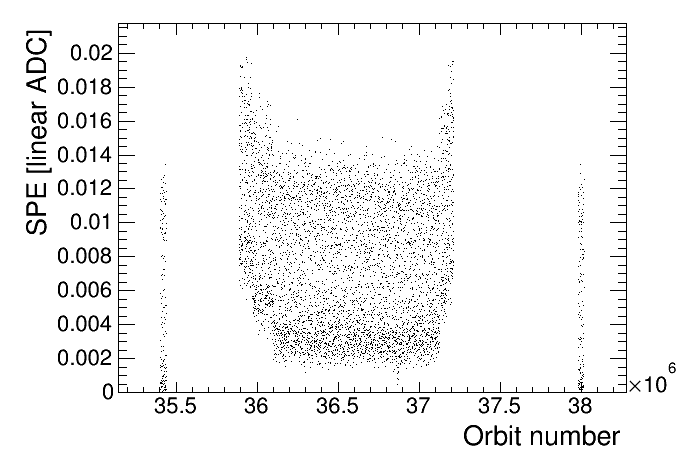
\includegraphics[width=0.6\textwidth]{fig/SPE_vs_ORN_unzoomed.png}
\begin{itemize}

\item Plot from Viktor Khristenko
\label{sec-1-1-1-2}%

\item Run: ???; Channel: HF(40, 23, 1)
\label{sec-1-1-1-3}%

\item \alert{Full} $x$-axis range shown
\label{sec-1-1-1-4}%
\end{itemize} % ends low level
\end{frame}
\begin{frame}
\frametitle{Issue: HF pedestal oscillating for some channels}
\label{sec-1-1-2}
%% Figure
\label{sec-1-1-2-1}

\centering
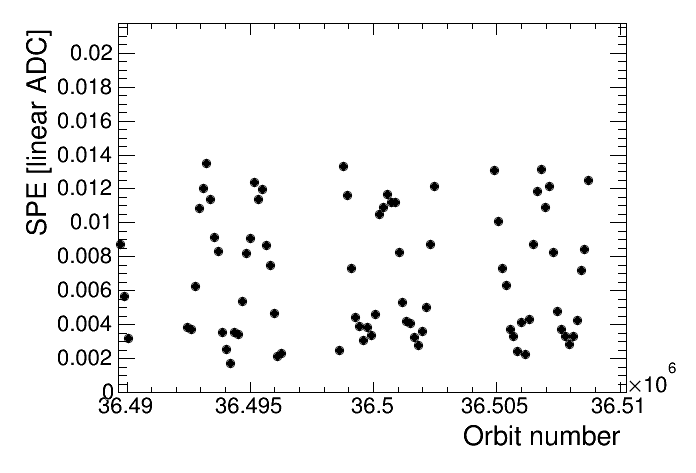
\includegraphics[width=0.6\textwidth]{fig/SPE_vs_ORN_zoomed.png}
\begin{itemize}

\item Same plot as last slide, but \alert{zoomed} $x$-axis range
\label{sec-1-1-2-2}%

\item Data broken into $0.35 s$ \alert{chunks} (expected)
\label{sec-1-1-2-3}%

\item Oscillations are clear (not in all channels)
\label{sec-1-1-2-4}%
\end{itemize} % ends low level
\end{frame}
\subsection{Goals}
\label{sec-1-2}
\begin{frame}
\frametitle{Goals}
\label{sec-1-2-1}
\begin{itemize}

\item Three (more?) main goals for this analysis:
\label{sec-1-2-1-1}%
\begin{enumerate}
\item Identify oscillating channels
\item Quantify oscillation
\item See if oscillation varies with time
\end{enumerate}

\item Focus on Goal 1 (identification) for now
\label{sec-1-2-1-2}%
\end{itemize} % ends low level
\end{frame}
\section{Method}
\label{sec-2}
\subsection{Method}
\label{sec-2-1}
\begin{frame}
\frametitle{Method: overview}
\label{sec-2-1-1}

\begin{enumerate}
\item Viktor provides a \texttt{TGraph} (slide 2) for each channel in run
\item For each channel, break \texttt{TGraph} into $0.35 s$ chunks
\item Convert each chunk's $x$-axis from OrN to time
\begin{itemize}
\item Divide OrN by orbit frequency in Hz
\end{itemize}
\item Fit each chunk ($\approx 200$) with a sinusoid
\item Use collection of fits to identify oscillating pedestals:
\begin{itemize}
\item Oscillating channels have good fits \& big amplitudes
\item Non-oscillating channels have bad fits \& low amplitudes
\end{itemize}
\end{enumerate}
\end{frame}
\begin{frame}
\frametitle{Method: the fit}
\label{sec-2-1-2}
\begin{itemize}

\item Fit function with 4 degrees of freedom:\\
\label{sec-2-1-2-1}%
\(f(t) = a_{0} + a_{1} \cdot \text{sin}(2\pi \cdot (f\cdot x + \phi))\)

\item Limits on parameters:
\label{sec-2-1-2-2}%
\begin{itemize}

\item Let $y_{i}$ be the SPE of the $i$-th point in the chunk
\label{sec-2-1-2-2-1}%
\begin{itemize}

\item $a_{0}$ varies between 0 and \(\left[2 \cdot \left(\frac{y_{\text{max}} + y_{\text{min}}}{2}\right)\right] \)
\label{sec-2-1-2-2-1-1}%

\item $a_{1}$ varies between 0 and \(\left[2 \cdot \left(\frac{y_{\text{max}} - y_{\text{min}}}{2}\right)\right] \)
\label{sec-2-1-2-2-1-2}%
\end{itemize} % ends low level

\item Let $f_{\text{FFT}}$ be the frequency found by the peak of an FFT on the chunk
\label{sec-2-1-2-2-2}%
\begin{itemize}

\item $f$ varies between 0 and sampling frequency
\label{sec-2-1-2-2-2-1}%

\item $f$ initially set to $f_{\text{FFT}}$
\label{sec-2-1-2-2-2-2}%
\end{itemize} % ends low level

\item No restrictions on phase
\label{sec-2-1-2-2-3}%
\begin{itemize}

\item $\phi$ varies between 0 and 1
\label{sec-2-1-2-2-3-1}%
\end{itemize} % ends low level
\end{itemize} % ends low level
\end{itemize} % ends low level
\end{frame}
\begin{frame}
\frametitle{Method: example on oscillating channel}
\label{sec-2-1-3}
\begin{columns} % Columns
\label{sec-2-1-3-1}
\begin{column}{0.55\textwidth}
%% Input histogram
\label{sec-2-1-3-1-1}

\centering
Example $0.35 s$ chunk input
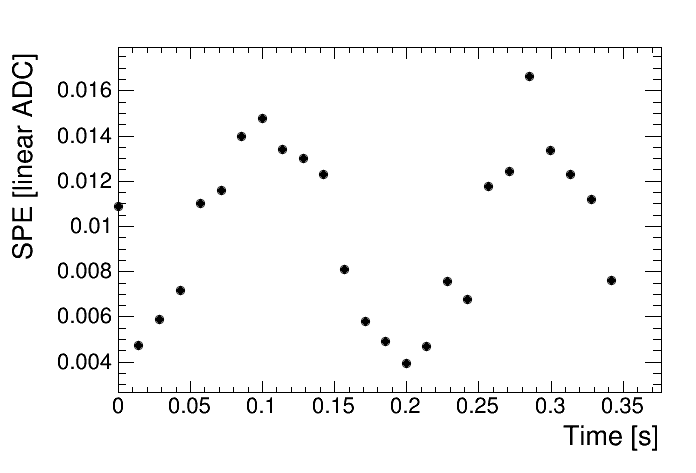
\includegraphics[width=.9\linewidth]{fig/input_graph_ieta40_iphi23_depth1.png}
\end{column}
\begin{column}{0.55\textwidth}
%% FFT output
\label{sec-2-1-3-1-2}

\centering
Example FFT output
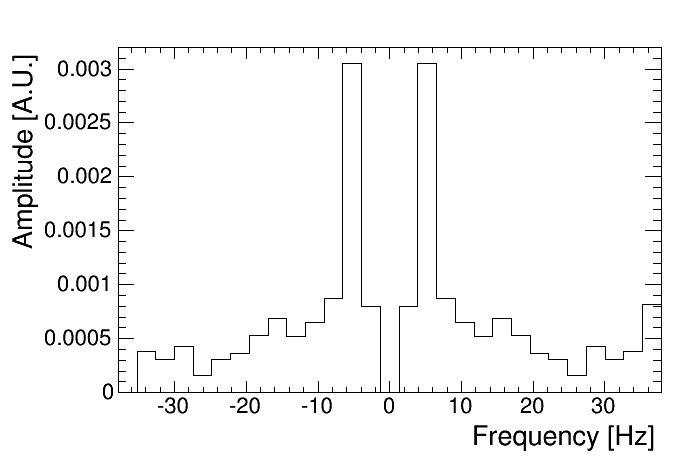
\includegraphics[width=.9\linewidth]{fig/fft_output_ieta40_iphi23_depth1.png}
\end{column}
\end{columns}
\begin{itemize}

\item Channel = HF(40, 23, 1): oscillating
\label{sec-2-1-3-2}%

\item FFT peaks around 5.2 Hz: $f$ is within [2.6, 10.4] Hz in fit
\label{sec-2-1-3-3}%

\item Fit on next slide
\label{sec-2-1-3-4}%
\end{itemize} % ends low level
\end{frame}
\begin{frame}
\frametitle{Method: example on oscillating channel}
\label{sec-2-1-4}
%% Figure
\label{sec-2-1-4-1}

\centering
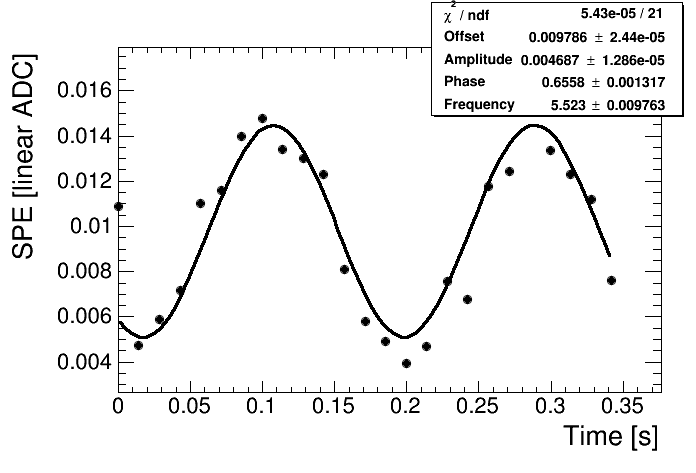
\includegraphics[width=0.6\textwidth]{fig/fit_output_ieta40_iphi23_depth1.png}
\begin{itemize}

\item Channel = HF(40, 23, 1): oscillating
\label{sec-2-1-4-2}%
\end{itemize} % ends low level
\end{frame}
\begin{frame}
\frametitle{Method: define fit significance}
\label{sec-2-1-5}
\begin{itemize}

\item Define variable to quantify residuals of data w.r.t. fit
\label{sec-2-1-5-1}%

\item Each point, $i$, in chunk has coordinate in time and SPE:
\label{sec-2-1-5-2}%
\begin{itemize}

\item time value: $t_i$ [s]
\label{sec-2-1-5-2-1}%

\item SPE value: $y_i$ [linear ADC]
\label{sec-2-1-5-2-2}%
\end{itemize} % ends low level

\item Fit function, $f$, is defined for each $t_i$
\label{sec-2-1-5-3}%

\item There are $N$ points in a given chunk
\label{sec-2-1-5-4}%

\item Define \alert{significance}, $\sigma$, for a chunk as follows:\\
\label{sec-2-1-5-5}%
\(\sigma = \frac{1}{N}\cdot\sqrt{\sum_{i=1}^{i=N}\left[f(t_{i}) - y_{i}\right]^{2}} \)
\begin{itemize}

\item $\sigma$ small for oscillating distributions
\label{sec-2-1-5-5-1}%

\item $\sigma$ large for non-oscillating distributions
\label{sec-2-1-5-5-2}%
\end{itemize} % ends low level
\end{itemize} % ends low level
\end{frame}
\begin{frame}
\frametitle{Method: example on oscillating channel}
\label{sec-2-1-6}
%% Figure
\label{sec-2-1-6-1}

\centering
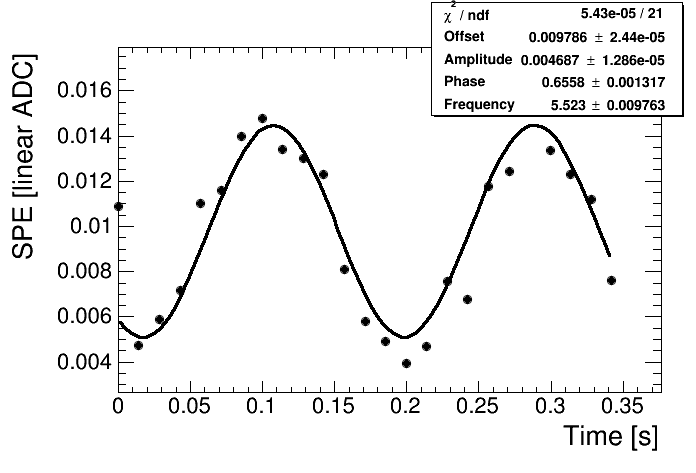
\includegraphics[width=0.6\textwidth]{fig/fit_output_ieta40_iphi23_depth1.png}
\begin{itemize}

\item Channel = HF(40, 23, 1): oscillating
\label{sec-2-1-6-2}%

\item $\sigma =$ 9.2e-5; $a_{1}$ (amplitude from fit) = 4.7e-3
\label{sec-2-1-6-3}%

\item \alert{$\sigma / a_{1} = 15.9$ (large)}
\label{sec-2-1-6-4}%
\end{itemize} % ends low level
\end{frame}
\begin{frame}
\frametitle{Method: example on non-oscillating channel}
\label{sec-2-1-7}
\begin{columns} % Columns
\label{sec-2-1-7-1}
\begin{column}{0.55\textwidth}
%% Input histogram
\label{sec-2-1-7-1-1}

\centering
Example $0.35 s$ chunk input
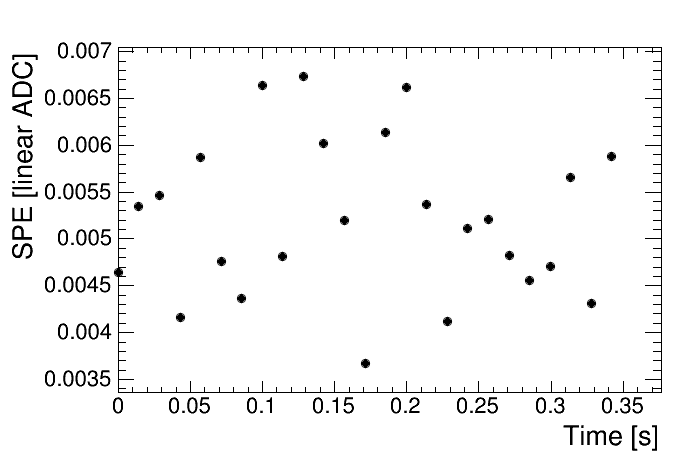
\includegraphics[width=.9\linewidth]{fig/input_graph_ieta38_iphi21_depth1.png}
\end{column}
\begin{column}{0.55\textwidth}
%% FFT output
\label{sec-2-1-7-1-2}

\centering
Example FFT output
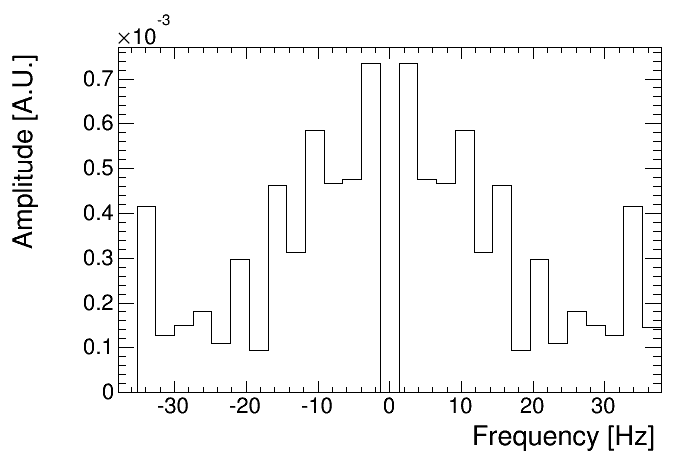
\includegraphics[width=.9\linewidth]{fig/fft_output_ieta38_iphi21_depth1.png}
\end{column}
\end{columns}
\begin{itemize}

\item Channel = HF(38, 21, 1): non-oscillating
\label{sec-2-1-7-2}%

\item FFT peaks around 2.6 Hz: $f$ is within [1.3, 5.2] Hz in fit
\label{sec-2-1-7-3}%

\item Fit on next slide
\label{sec-2-1-7-4}%
\end{itemize} % ends low level
\end{frame}
\begin{frame}
\frametitle{Method: example on non-oscillating channel}
\label{sec-2-1-8}
%% Figure
\label{sec-2-1-8-1}

\centering
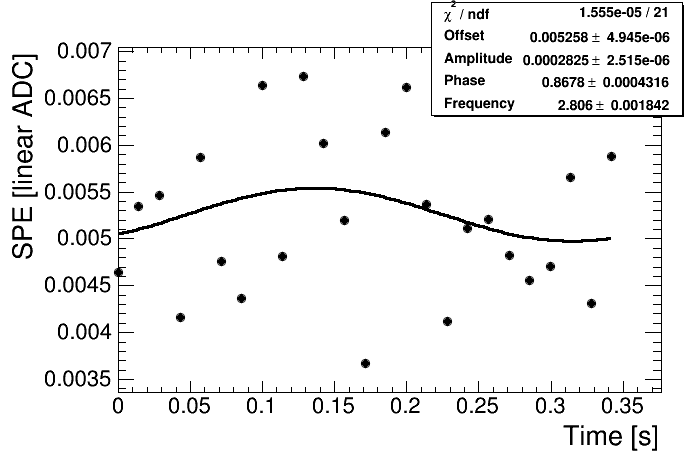
\includegraphics[width=0.6\textwidth]{fig/fit_output_ieta38_iphi21_depth1.png}
\begin{itemize}

\item Channel = HF(38, 21, 1): non-oscillating
\label{sec-2-1-8-2}%

\item $\sigma =$ 1.6e-4; $a_{1}$ (amplitude from fit) = 2.8e-4
\label{sec-2-1-8-3}%

\item \alert{$\sigma / a_{1} = 1.8$ (small)}
\label{sec-2-1-8-4}%
\end{itemize} % ends low level
\end{frame}
\begin{frame}
\frametitle{Method: look at all $0.35 s$ chunks for two channels}
\label{sec-2-1-9}
%% Figure
\label{sec-2-1-9-1}

\centering
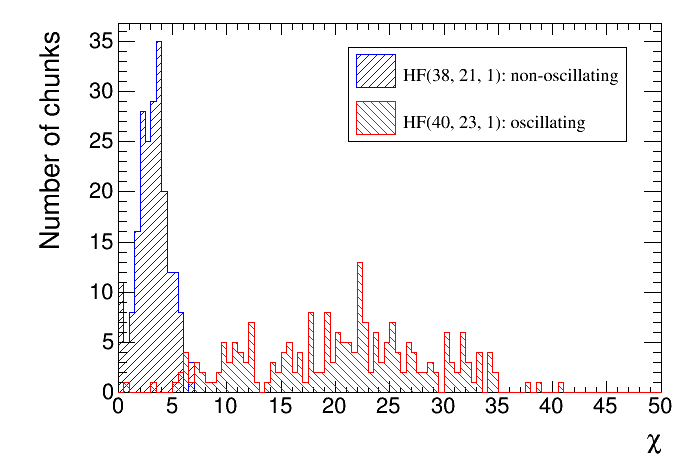
\includegraphics[width=0.6\textwidth]{fig/amp_over_signif_comparison.png}
\begin{itemize}

\item Define \alert{$\chi = \sigma / a_{1}$}: a good measure for ``oscillating-ness''
\label{sec-2-1-9-2}%

\item Naively look for chunks with $\chi > 10$
\label{sec-2-1-9-3}%

\item Enough method: let's look at results
\label{sec-2-1-9-4}%
\end{itemize} % ends low level
\end{frame}
\section{Results}
\label{sec-3}
\subsection{Time vs. Frequency}
\label{sec-3-1}
\begin{frame}
\frametitle{Results: $\chi$ vs. time for all chunks}
\label{sec-3-1-1}
%% Figure
\label{sec-3-1-1-1}

\centering
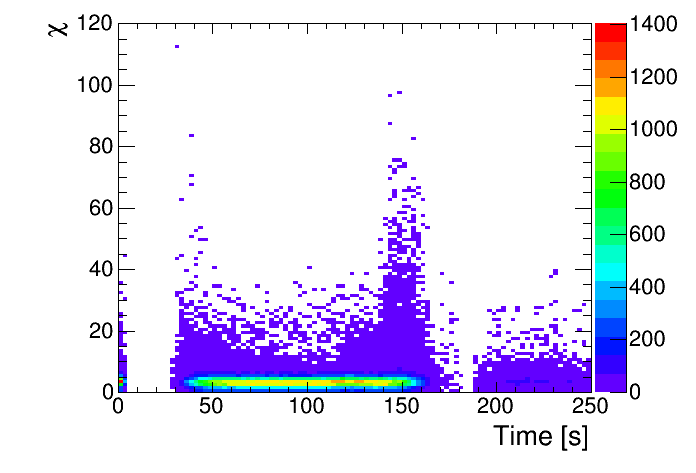
\includegraphics[width=0.6\textwidth]{fig/time_vs_amp_over_significance_hist.png}
\begin{itemize}

\item Plot is a 2D histogram
\label{sec-3-1-1-2}%

\item One entry per chunk, per channel
\label{sec-3-1-1-3}%

\item $x$-axis: time [seconds], $y$-axis: $\chi$
\label{sec-3-1-1-4}%
\end{itemize} % ends low level
\end{frame}
\begin{frame}
\frametitle{Results: Freq. vs. time for chunks with $\chi > 10$}
\label{sec-3-1-2}
%% Figure
\label{sec-3-1-2-1}

\centering
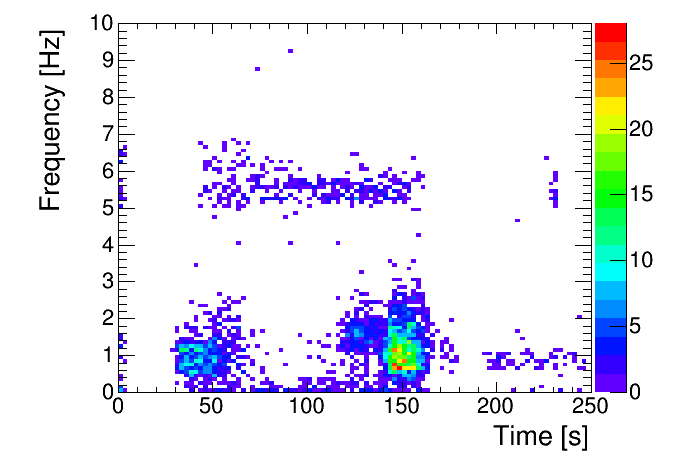
\includegraphics[width=0.6\textwidth]{fig/time_vs_frequency_signifOver10_hist.png}
\begin{itemize}

\item Plot is a 2D histogram
\label{sec-3-1-2-2}%

\item One entry per chunk, per channel, \alert{if chunk $\chi > 10$}
\label{sec-3-1-2-3}%

\item $x$-axis: time [seconds], $y$-axis: frequency from fit
\label{sec-3-1-2-4}%
\end{itemize} % ends low level
\end{frame}
\begin{frame}
\frametitle{Observations:}
\label{sec-3-1-3}
\begin{itemize}

\item Observations from the $\chi$ vs time plot:
\label{sec-3-1-3-1}%
\begin{itemize}

\item Most chunks have $\chi < 10$ (non-oscillating)
\label{sec-3-1-3-1-1}%

\item There are spikes in $\chi$ at time = 40s and 150s
\label{sec-3-1-3-1-2}%
\end{itemize} % ends low level

\item Observations from the frequency vs time plot:
\label{sec-3-1-3-2}%
\begin{itemize}

\item \alert{Two frequencies of oscillation observed}
\label{sec-3-1-3-2-1}%

\item Spikes in $\chi$ at time = 40s and 150s are mostly 0-2 Hz
\label{sec-3-1-3-2-2}%

\item Roughly constant rate of 5-7 Hz chunks between \\ time = 40s and 150s
\label{sec-3-1-3-2-3}%
\end{itemize} % ends low level

\item Next:
\label{sec-3-1-3-3}%
\begin{itemize}

\item Where (ieta, iphi, depth) are the 0-2 Hz chunks?
\label{sec-3-1-3-3-1}%

\item Where (ieta, iphi, depth) are the 5-7 Hz chunks?
\label{sec-3-1-3-3-2}%
\end{itemize} % ends low level
\end{itemize} % ends low level
\end{frame}
\subsection{0-2 Hz chunks}
\label{sec-3-2}
\begin{frame}
\frametitle{Results: Where are the 0-2 Hz chunks (30-60 s)?}
\label{sec-3-2-1}
\begin{columns} % Columns
\label{sec-3-2-1-1}
\begin{column}{0.55\textwidth}
%% Depth 1
\label{sec-3-2-1-1-1}

\centering
Occupancy, Depth = 1
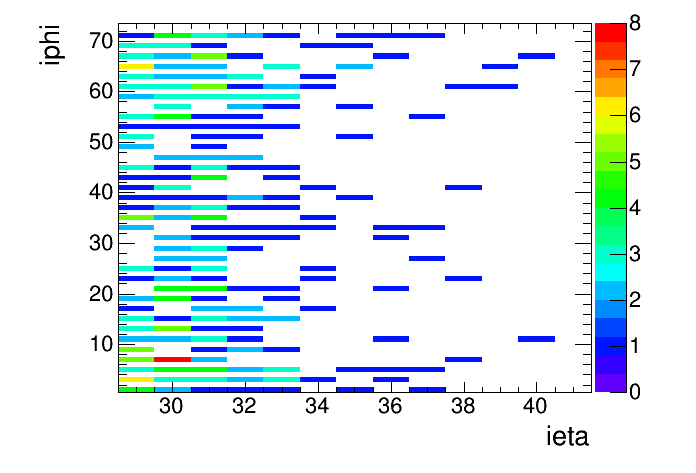
\includegraphics[width=\textwidth]{fig/occupancy_frequencyUnder4_time30to60_signifOver10_depth1_hist.png}
\end{column}
\begin{column}{0.55\textwidth}
%% Depth 2
\label{sec-3-2-1-1-2}

\centering
Occupancy, Depth = 2
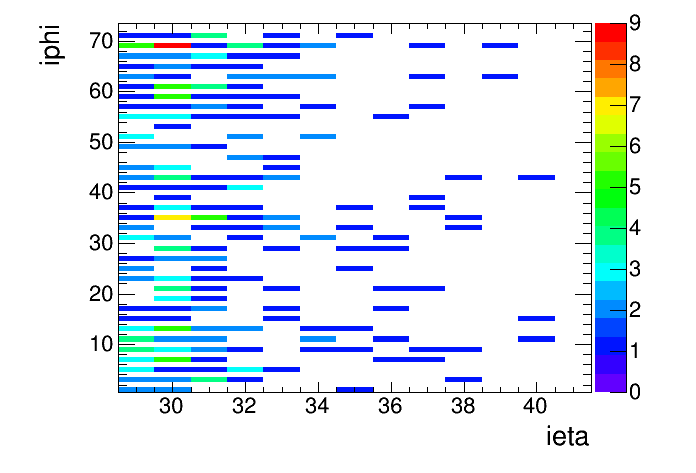
\includegraphics[width=\textwidth]{fig/occupancy_frequencyUnder4_time30to60_signifOver10_depth2_hist.png}
\end{column}
\end{columns}
\begin{itemize}

\item Plot is a 2D histogram
\label{sec-3-2-1-2}%

\item One entry per chunk, per channel,\\ \alert{if freq $< 4$ Hz, $\chi > 10$, and time $\epsilon$ [30, 60]}
\label{sec-3-2-1-3}%

\item $x$-axis: ieta, $y$-axis: iphi
\label{sec-3-2-1-4}%
\end{itemize} % ends low level
\end{frame}
\begin{frame}
\frametitle{Results: Where are the 0-2 Hz chunks (140-160 s)?}
\label{sec-3-2-2}
\begin{columns} % Columns
\label{sec-3-2-2-1}
\begin{column}{0.55\textwidth}
%% Depth 1
\label{sec-3-2-2-1-1}

\centering
Occupancy, Depth = 1
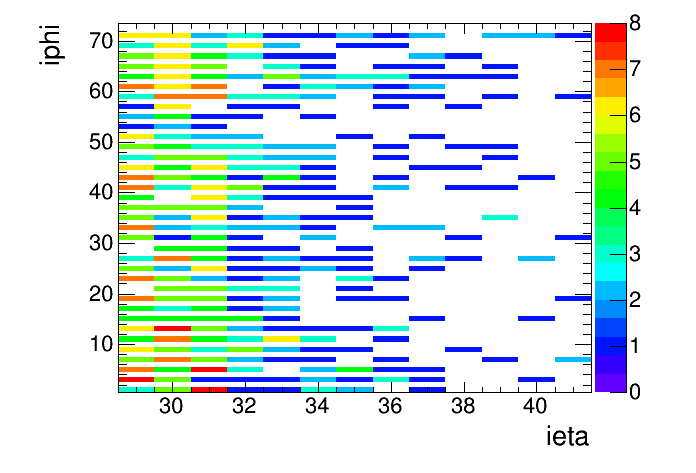
\includegraphics[width=\textwidth]{fig/occupancy_frequencyUnder4_time140to160_signifOver10_depth1_hist.png}
\end{column}
\begin{column}{0.55\textwidth}
%% Depth 2
\label{sec-3-2-2-1-2}

\centering
Occupancy, Depth = 2
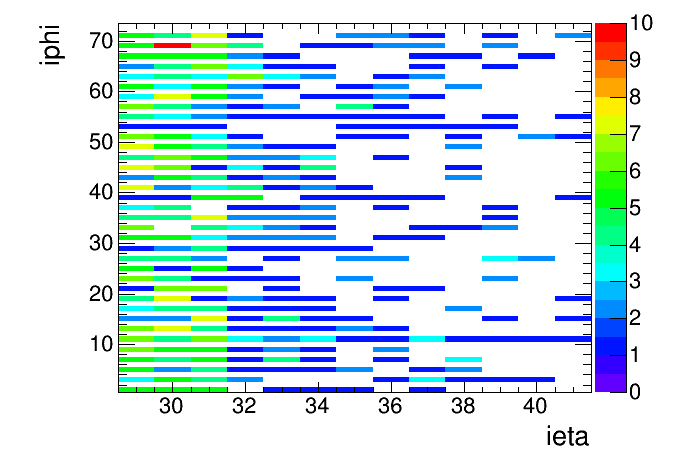
\includegraphics[width=\textwidth]{fig/occupancy_frequencyUnder4_time140to160_signifOver10_depth2_hist.png}
\end{column}
\end{columns}
\begin{itemize}

\item Plot is a 2D histogram
\label{sec-3-2-2-2}%

\item One entry per chunk, per channel,\\ \alert{if freq $< 4$ Hz, $\chi > 10$, and time $\epsilon$ [140, 160]}
\label{sec-3-2-2-3}%

\item $x$-axis: ieta, $y$-axis: iphi
\label{sec-3-2-2-4}%
\end{itemize} % ends low level
\end{frame}
\begin{frame}
\frametitle{Results: What does an 0-2 Hz chunk look like?}
\label{sec-3-2-3}
%% Figure
\label{sec-3-2-3-1}

\centering
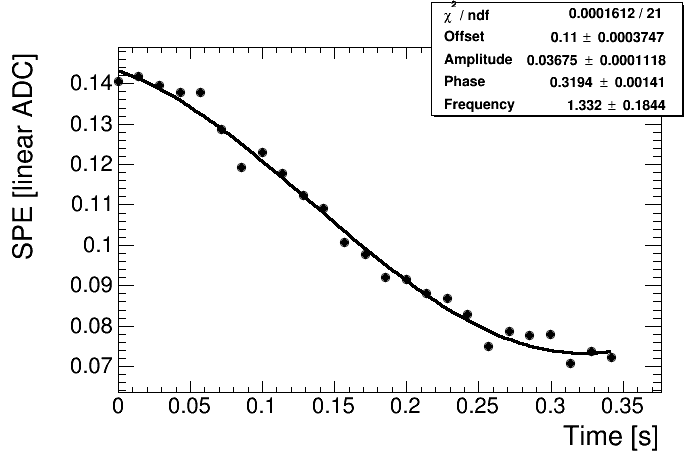
\includegraphics[width=0.6\textwidth]{fig/fit_output_ieta29_iphi5_depth1_burst199.png}
\begin{itemize}

\item Channel: HF(29, 5, 1)
\label{sec-3-2-3-2}%

\item Time: 145s
\label{sec-3-2-3-3}%

\item Frequency: $1.3 \pm 0.2$ Hz
\label{sec-3-2-3-4}%
\end{itemize} % ends low level
\end{frame}
\begin{frame}
\frametitle{Observations: 0-2 Hz chunks}
\label{sec-3-2-4}
\begin{itemize}

\item 0-2 Hz chunks more common at 140-160 than at 30-60 s
\label{sec-3-2-4-1}%

\item No single channel contributing most of the 0-2 Hz chunks
\label{sec-3-2-4-2}%

\item Low-ieta channels are far more likely to have 0-2 Hz chunks
\label{sec-3-2-4-3}%

\item Side effect from sourcing?
\label{sec-3-2-4-4}%
\end{itemize} % ends low level
\end{frame}
\subsection{5-7 Hz chunks}
\label{sec-3-3}
\begin{frame}
\frametitle{Results: Where are the 5-7 Hz chunks?}
\label{sec-3-3-1}
\begin{columns} % Columns
\label{sec-3-3-1-1}
\begin{column}{0.55\textwidth}
%% Depth 1
\label{sec-3-3-1-1-1}

\centering
Occupancy, Depth = 1
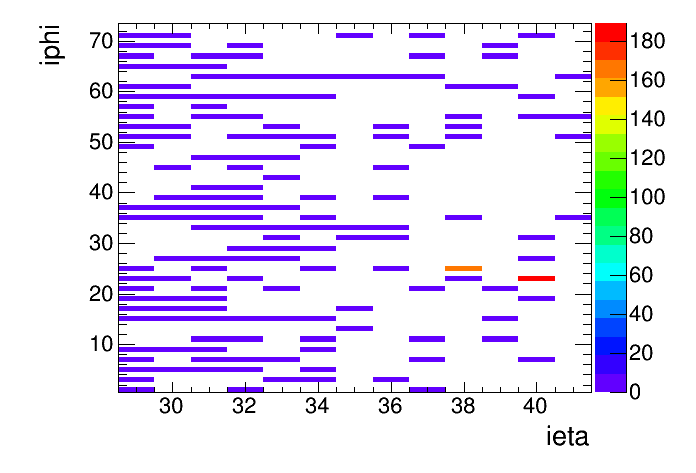
\includegraphics[width=\textwidth]{fig/occupancy_frequencyOver4_signifOver10_depth1_hist.png}
\end{column}
\begin{column}{0.55\textwidth}
%% Depth 2
\label{sec-3-3-1-1-2}

\centering
Occupancy, Depth = 2
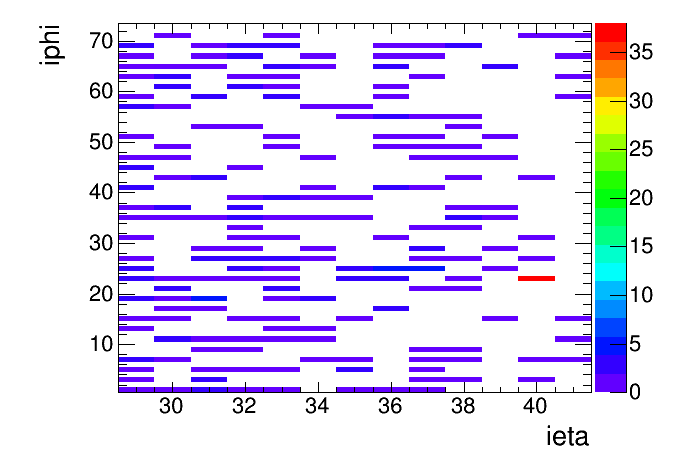
\includegraphics[width=\textwidth]{fig/occupancy_frequencyOver4_signifOver10_depth2_hist.png}
\end{column}
\end{columns}
\begin{itemize}

\item Plot is a 2D histogram
\label{sec-3-3-1-2}%

\item One entry per chunk, per channel,\\ \alert{if freq $> 4$ Hz and $\chi > 10$}
\label{sec-3-3-1-3}%

\item $x$-axis: ieta, $y$-axis: iphi
\label{sec-3-3-1-4}%
\end{itemize} % ends low level
\end{frame}
\begin{frame}
\frametitle{Observations:}
\label{sec-3-3-2}
\begin{itemize}

\item 5-7 Hz chunks mostly come from three \alert{hot} channels:
\label{sec-3-3-2-1}%
\begin{itemize}

\item HF(40, 23, 1)
\label{sec-3-3-2-1-1}%

\item HF(40, 23, 2)
\label{sec-3-3-2-1-2}%

\item HF(38, 25, 1)
\label{sec-3-3-2-1-3}%
\end{itemize} % ends low level

\item Other channels contribute relatively few chunks per run
\label{sec-3-3-2-2}%

\item Next:
\label{sec-3-3-2-3}%
\begin{itemize}

\item More investigation into these oscillating channels
\label{sec-3-3-2-3-1}%

\item Compare against HF(38, 21, 1) (non-oscillating)
\label{sec-3-3-2-3-2}%
\end{itemize} % ends low level
\end{itemize} % ends low level
\end{frame}
\begin{frame}
\frametitle{Results: $\left<\chi\right>$ for 5-7 Hz hot channels}
\label{sec-3-3-3}
%% Figure
\label{sec-3-3-3-1}

\centering
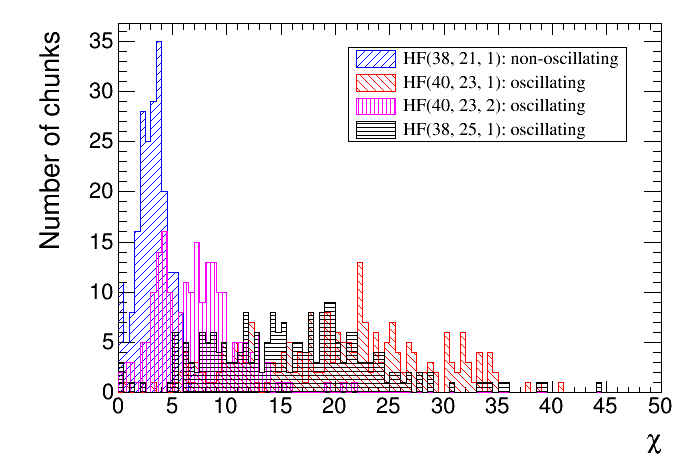
\includegraphics[width=0.6\textwidth]{fig/amp_over_signif_comparison_more.png}
\begin{itemize}

\item HF(40, 23, 1): $\left<\chi\right> = 21.2$
\label{sec-3-3-3-2}%

\item HF(38, 25, 1): $\left<\chi\right> = 17.2$
\label{sec-3-3-3-3}%

\item HF(40, 23, 2): $\left<\chi\right> = 7.2$
\label{sec-3-3-3-4}%
\end{itemize} % ends low level
\end{frame}
\begin{frame}
\frametitle{Results: Amplitude and Frequency HF(38, 21, 1)}
\label{sec-3-3-4}
\begin{columns} % Columns
\label{sec-3-3-4-1}
\begin{column}{0.55\textwidth}
%% Amplitude
\label{sec-3-3-4-1-1}

\centering
Amplitude from fit
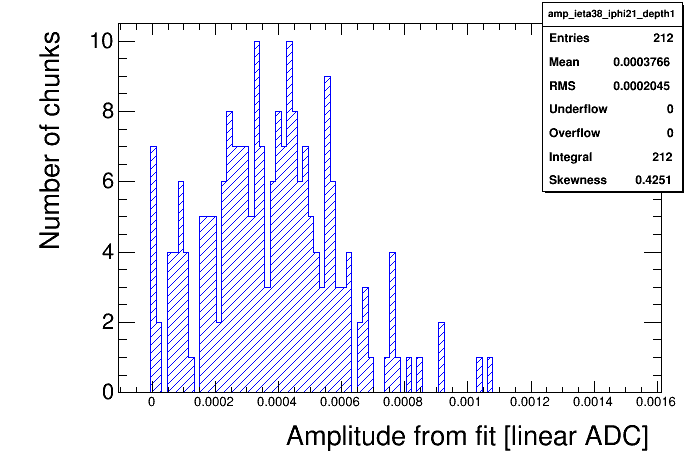
\includegraphics[width=.9\linewidth]{fig/amp_ieta38_iphi21_depth1.png}
\end{column}
\begin{column}{0.55\textwidth}
%% Frequency
\label{sec-3-3-4-1-2}

\centering
Frequency from fit
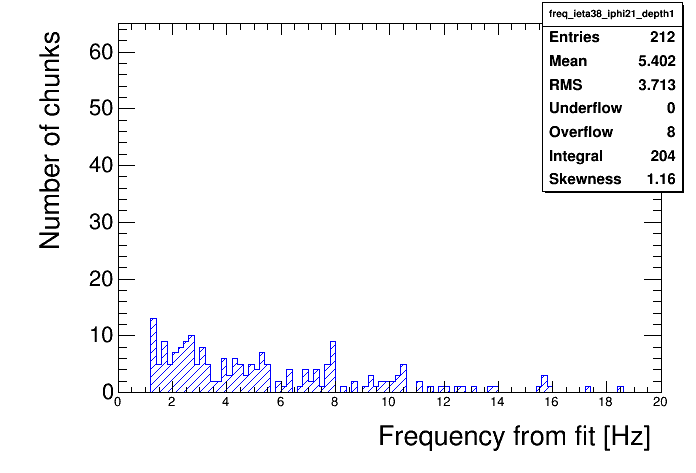
\includegraphics[width=.9\linewidth]{fig/freq_ieta38_iphi21_depth1.png}
\end{column}
\end{columns}
\begin{itemize}

\item \alert{Non-oscillating} channel
\label{sec-3-3-4-2}%

\item Avg. amplitude = $0.00038 \pm 0.00020$
\label{sec-3-3-4-3}%
\end{itemize} % ends low level
\end{frame}
\begin{frame}
\frametitle{Results: Amplitude and Frequency HF(40, 23, 1)}
\label{sec-3-3-5}
\begin{columns} % Columns
\label{sec-3-3-5-1}
\begin{column}{0.55\textwidth}
%% Amplitude
\label{sec-3-3-5-1-1}

\centering
Amplitude from fit
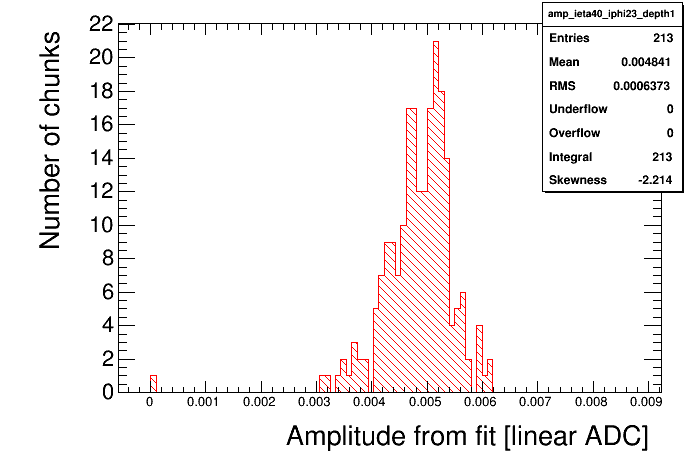
\includegraphics[width=.9\linewidth]{fig/amp_ieta40_iphi23_depth1.png}
\end{column}
\begin{column}{0.55\textwidth}
%% Frequency
\label{sec-3-3-5-1-2}

\centering
Frequency from fit
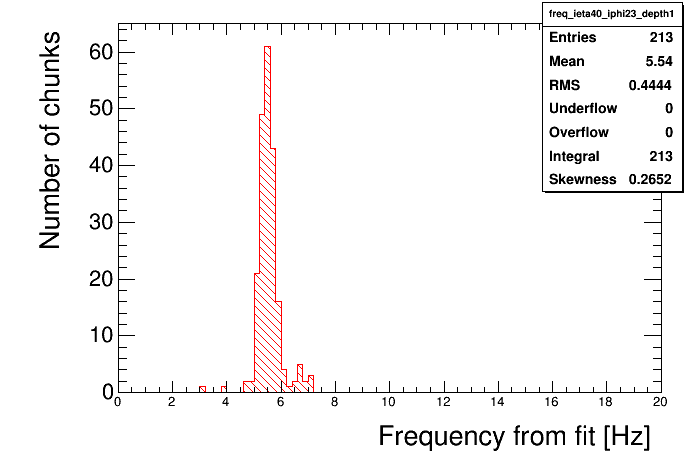
\includegraphics[width=.9\linewidth]{fig/freq_ieta40_iphi23_depth1.png}
\end{column}
\end{columns}
\begin{itemize}

\item \alert{Oscillating} channel
\label{sec-3-3-5-2}%

\item Avg. amplitude = $0.00484 \pm 0.00064$
\label{sec-3-3-5-3}%

\item Avg. frequency = $5.54 \pm 0.44$
\label{sec-3-3-5-4}%
\end{itemize} % ends low level
\end{frame}
\begin{frame}
\frametitle{Results: Amplitude and Frequency HF(40, 23, 2)}
\label{sec-3-3-6}
\begin{columns} % Columns
\label{sec-3-3-6-1}
\begin{column}{0.55\textwidth}
%% Amplitude
\label{sec-3-3-6-1-1}

\centering
Amplitude from fit
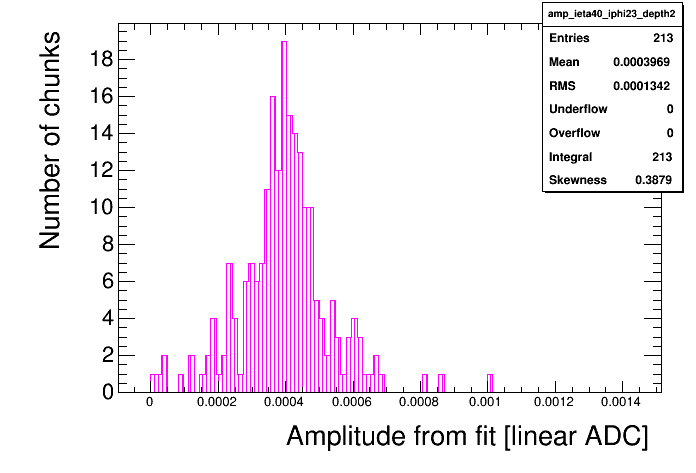
\includegraphics[width=.9\linewidth]{fig/amp_ieta40_iphi23_depth2.png}
\end{column}
\begin{column}{0.55\textwidth}
%% Frequency
\label{sec-3-3-6-1-2}

\centering
Frequency from fit
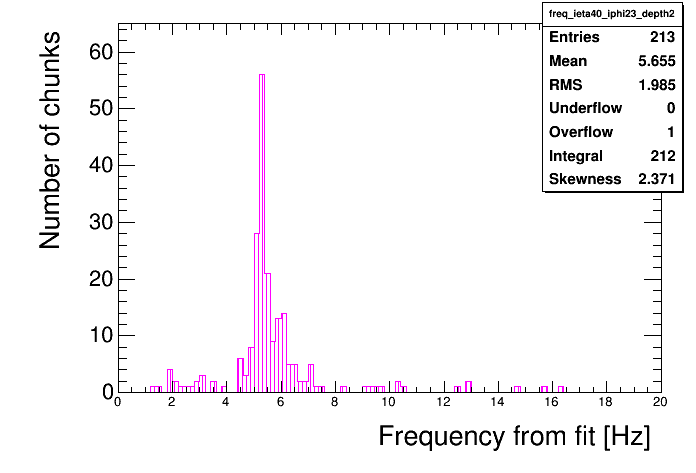
\includegraphics[width=.9\linewidth]{fig/freq_ieta40_iphi23_depth2.png}
\end{column}
\end{columns}
\begin{itemize}

\item \alert{Oscillating} channel
\label{sec-3-3-6-2}%

\item Avg. amplitude = $0.00040 \pm 0.00013$
\label{sec-3-3-6-3}%

\item Avg. frequency = $5.65 \pm 1.99$
\label{sec-3-3-6-4}%
\end{itemize} % ends low level
\end{frame}
\begin{frame}
\frametitle{Results: Amplitude and Frequency HF(38, 25, 1)}
\label{sec-3-3-7}
\begin{columns} % Columns
\label{sec-3-3-7-1}
\begin{column}{0.55\textwidth}
%% Amplitude
\label{sec-3-3-7-1-1}

\centering
Amplitude from fit
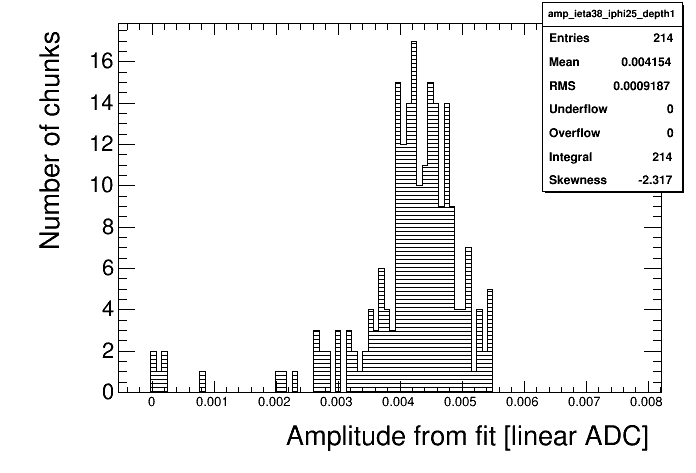
\includegraphics[width=.9\linewidth]{fig/amp_ieta38_iphi25_depth1.png}
\end{column}
\begin{column}{0.55\textwidth}
%% Frequency
\label{sec-3-3-7-1-2}

\centering
Frequency from fit
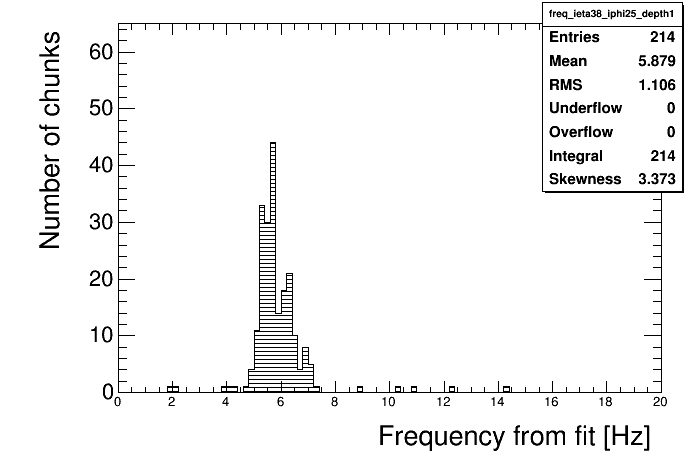
\includegraphics[width=.9\linewidth]{fig/freq_ieta38_iphi25_depth1.png}
\end{column}
\end{columns}
\begin{itemize}

\item \alert{Oscillating} channel
\label{sec-3-3-7-2}%

\item Avg. amplitude = $0.00415 \pm 0.00092$
\label{sec-3-3-7-3}%

\item Avg. frequency = $5.88 \pm 1.11$
\label{sec-3-3-7-4}%
\end{itemize} % ends low level
\end{frame}
\begin{frame}
\frametitle{Results: Amplitude and Frequency observations}
\label{sec-3-3-8}
\begin{itemize}

\item Avg. amplitudes of oscillating channels vary by an order of magnitude:
\label{sec-3-3-8-1}%
\begin{itemize}

\item Avg. amplitude = $0.00484 \pm 0.00064$ in HF(40, 23, 1)
\label{sec-3-3-8-1-1}%

\item Avg. amplitude = $0.00040 \pm 0.00013$ in HF(40, 23, 2)
\label{sec-3-3-8-1-2}%

\item Units are linear ADC ($y$-axis of Viktor's plots)
\label{sec-3-3-8-1-3}%
\end{itemize} % ends low level
\end{itemize} % ends low level
\end{frame}
\section{Conclusions}
\label{sec-4}
\subsection{Conclusions}
\label{sec-4-1}
\subsection{Conclusions}
\label{sec-4-2}
\begin{frame}
\frametitle{Conclusions}
\label{sec-4-2-1}
\begin{itemize}

\item Used $\chi$ to find oscillating channels
\label{sec-4-2-1-1}%
\begin{itemize}

\item Variable determined from FFT + sine-wave fit
\label{sec-4-2-1-1-1}%
\end{itemize} % ends low level

\item Found two kinds of oscillations:
\label{sec-4-2-1-2}%
\begin{itemize}

\item 0-2 Hz, spread in low-ieta channels at specific times
\label{sec-4-2-1-2-1}%
\begin{itemize}

\item Related to movement of the source?
\label{sec-4-2-1-2-1-1}%
\end{itemize} % ends low level

\item 5-7 Hz, mostly from three hot channels at all times:
\label{sec-4-2-1-2-2}%
\begin{itemize}

\item HF(40, 23, 1)
\label{sec-4-2-1-2-2-1}%

\item HF(40, 23, 2)
\label{sec-4-2-1-2-2-2}%

\item HF(38, 25, 1)
\label{sec-4-2-1-2-2-3}%
\end{itemize} % ends low level
\end{itemize} % ends low level

\item 5-7 Hz chunks have widely varying amplitudes:
\label{sec-4-2-1-3}%
\begin{itemize}

\item Avg. amplitude = $0.00484 \pm 0.00064$ in HF(40, 23, 1)
\label{sec-4-2-1-3-1}%

\item Avg. amplitude = $0.00040 \pm 0.00013$ in HF(40, 23, 2)
\label{sec-4-2-1-3-2}%
\end{itemize} % ends low level
\end{itemize} % ends low level
\end{frame}
\section{Backup}
\label{sec-5}
\subsection{Backup}
\label{sec-5-1}
\begin{frame}
\frametitle{Backup: Mean $\chi$}
\label{sec-5-1-1}
\begin{columns} % Columns
\label{sec-5-1-1-1}
\begin{column}{0.55\textwidth}
%% Figure
\label{sec-5-1-1-1-1}

\centering
$\left<\chi\right>$, Depth = 1 \\
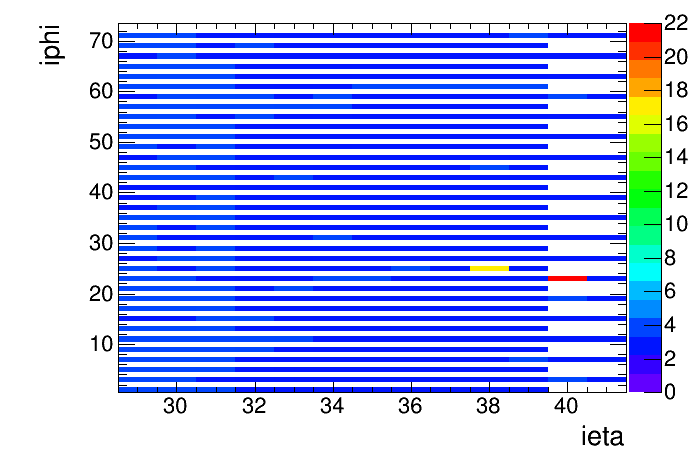
\includegraphics[width=\textwidth]{fig/mean_fit_amp_over_significance_depth1_hist.png}
\end{column}
\begin{column}{0.55\textwidth}
%% Figure
\label{sec-5-1-1-1-2}

\centering
$\left<\chi\right>$, Depth = 2 \\
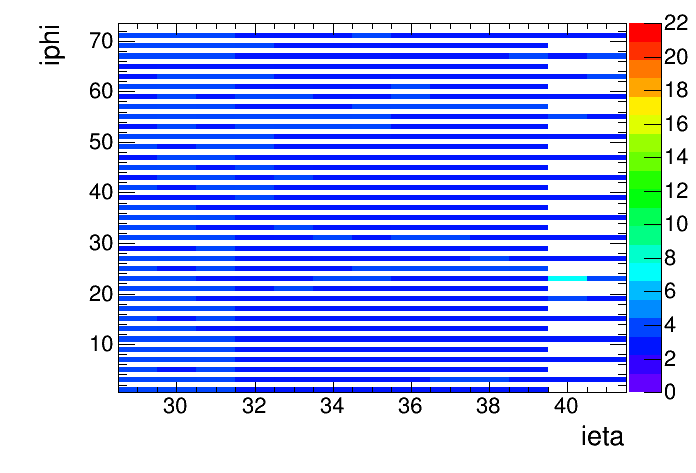
\includegraphics[width=\textwidth]{fig/mean_fit_amp_over_significance_depth2_hist.png}
\end{column}
\end{columns}
\begin{itemize}

\item HF(40, 23, 1): $\left<\sigma / a_{1}\right> = 21.2$
\label{sec-5-1-1-2}%

\item HF(38, 25, 1): $\left<\sigma / a_{1}\right> = 17.2$
\label{sec-5-1-1-3}%

\item HF(40, 23, 2): $\left<\sigma / a_{1}\right> = 7.2$
\label{sec-5-1-1-4}%
\end{itemize} % ends low level
\end{frame}

\end{document}
